\documentclass[letterpaper, 12pt]{article}
\usepackage[]{graphicx}
\usepackage[]{color} % use "amsart" instead of "article" for AMSLaTeX format
\usepackage{geometry}                % See geometry.pdf to learn the layout options. There are lots.
\geometry{letterpaper}                     % ... or a4paper or a5paper or ... 
\usepackage[notocbib]{apacite}
%\usepackage{subfigure}
%\usepackage{alltt}
%\usepackage{etex}     
%\usepackage{amsfonts, amsmath, amssymb, latexsym, mathrsfs, fancyhdr,theorem,  pifont, setspace, verbatim,  qtree, lscape, tipa, linguex, hyperref, wasysym, stmaryrd, natbib,soul, minibox, lipsum, setspace, amssymb, color, multirow, multicol, soul,geometry,graphicx, wrapfig,gb4e,booktabs}
%\usepackage[T1]{fontenc}
%\usepackage{times}
%\usepackage{helvet}
%\renewcommand{\familydefault}{\sfdefault}
\geometry{hmargin={1in,1in},vmargin={1in,1in}}
\definecolor{Red}{RGB}{255,0,0}
\graphicspath{{figs/}}
\usepackage{amssymb,amsmath}
\usepackage{gensymb}
\usepackage{csquotes}
\newcommand{\denote}[1]{\mbox{ $[\![ #1 ]\!]$}}
\usepackage{tikz}
\usepackage{tikz-qtree}
\usepackage{caption}
\usepackage{wrapfig}
\usepackage{pslatex}
\usepackage{apacite}
\usepackage{amsmath}
\usepackage{float} % Roger Levy added this and changed figure/table
                   % placement to [H] for conformity to Word template,
                   % though floating tables and figures to top is
                   % still generally recommended!

%\title{Brief Article}
%\author{Authors}
%\date{ % Activate to display a given date or no date


\begin{document}
\begin{center}
\textbf{Comparison class inference for gradable adjectives}
\end{center}

A 24 \degree C  (75 \degree F) day is warm, while a 16 \degree C  (60 \degree F) day is not. Unless it's January. 16 \degree C  could be warm for January.
\emph{Warm} is a relative adjective, and its felicity depends upon what the speaker uses as a basis of comparison---the \emph{comparison class} (e.g., other days of the year~vs,~January).
Comparison classes are necessary for understanding gradable adjectives, but as with relevant aspects of context more generally, comparison classes often go unsaid (e.g., in ``It's warm'').

% and, in fact, any part of language whose meaning must be pragmatically reconstructed from context, including vague quantifiers \cite<e.g., ``He ate a lot of burgers''; >{Scholler2017} and generic language \cite<e.g., ``Dogs are friendly''; >{Tessler2019psychrev}.
%%Deciding on the relevant comparison class is a case study in the larger question of inferring the appropriate aspects of context for interpreting an utterance.
%The trouble is:

How do listeners decide on the appropriate comparison class? 
Any particular referent of discourse can be conceptualized or categorized in multiple ways, giving rise to multiple possible comparison classes: 
%A day in January is also a day of the year; if a listener hear \enquote{It's warm}, it could be \emph{warm for the week}, \emph{warm for winter}, or \emph{warm for the year}, among many other possibilities.
In this project, we investigate the first aspect of this open-ended inference problem: deciding between a relatively specific comparison class (e.g., \emph{warm for winter}) and a relatively general class (e.g., \emph{warm for the year}).
Theoretical work in semantics has focused on how information from the comparison class gets integrated with a compositional semantics and what representations might be preferred \cite{Bale2011, Solt2009}. 
To our knowledge, the question of how listeners reconstruct a comparison class from just the adjective and world knowledge has not been addressed either empirically or  formally.

\begin{wrapfigure}{r}{0.43\textwidth}
\vspace{-1cm}
  \begin{center}
    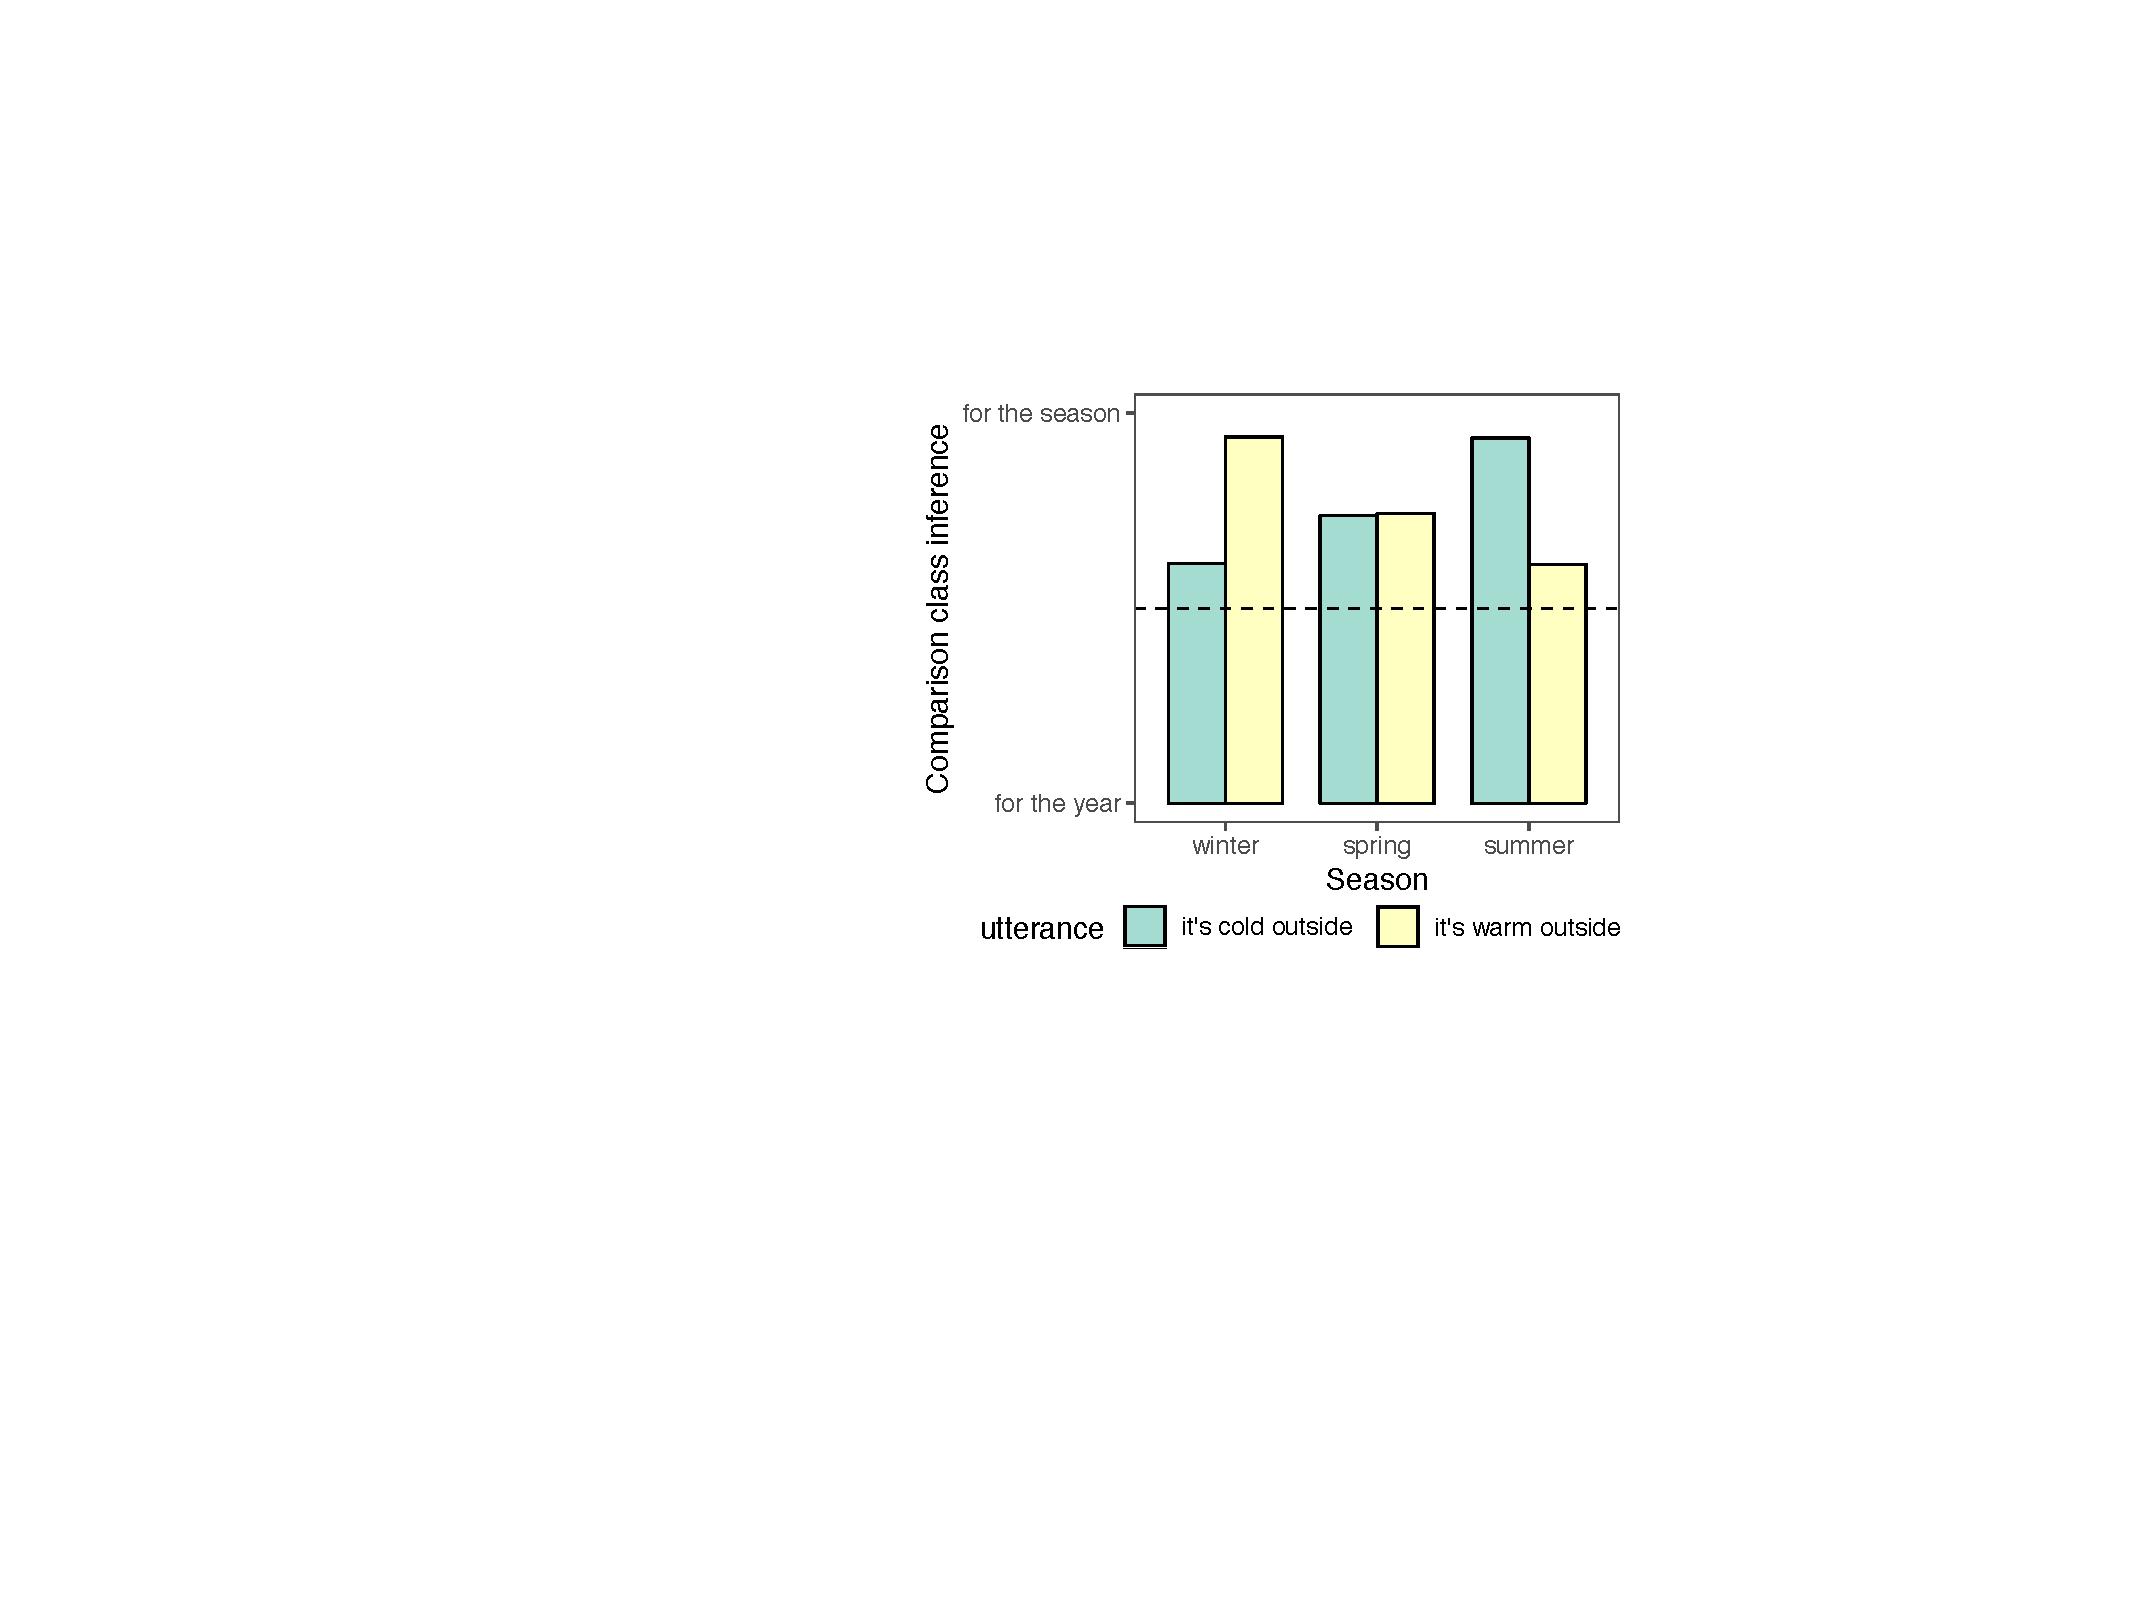
\includegraphics[width=0.43\textwidth]{L1preds}
  \end{center}
  \vspace{-0.45cm}
  \caption{\small 
%  Speaker model behavior assuming
%different comparison classes. The underspecified utterance
%(\enquote{warm}) takes on the same meaning of the explicit utterance
%whose comparison class is the same as the implicit class (e.g., if the
%speaker is using the (for winter) comparison class, \enquote{warm} means
%the same thing as \enquote{warm for winter}). When the speaker is
%assuming winter is the comparison class, when the temperture is low, she
%will say \enquote{warm} or \enquote{warm for winter}, but if the
%temperature is relatively high, she will only say \enquote{warm for the
%year}. When the speaker is assuming the year is the comparison class,
%and the temperature is relatively low, she will say \enquote{warm for
%winter}. The listener believes temperature is relatively low (believes
%it is winter), and inverts this model of speaker to conclude that the
%implicit comparison class was winter. The specific class in this example
%(winter) is a Normal distribution centered at -1, and the general class
%(the year) is a Normal centered at 0.
Listener inferences about the comparison class  upon  hearing either a positive-form adjective (``warm'') or negative-form adjective (''cold'') during different seasons. 
  }
  \vspace{-0.55cm}
  \label{fig:predictions}
\end{wrapfigure}


We develop a Rational Speech Act model wherein a listener combines hierarchical, category knowledge with pragmatic reasoning to infer the comparison class implicitly used by the speaker.
The model combines a previously proposed method for inferring common ground \cite{Degen2015} with an uncertain threshold mechanism for deriving context-sensitive interpretations for gradable adjectives \cite{Lassiter2015}.
%We model a situation in which a listener hears just an adjective (``it's warm'') and tries to reconstruct the comparison class. 
In this model, the speaker could have produced an adjective with an explicit comparison class (``warm for winter''), which has the effect of changing the common ground (or, the listener's prior distribution over the degree e.g., temperature).
In this way, reasoning about the comparison class is cashed out in terms of reasoning about alternative utterances (in this case, alternative utterances using different comparison classes).
The model predicts that hearing \enquote{it's warm} (in Winter) signals that the speaker meant \emph{warm for winter}, while hearing \enquote{it's cold} is more likely to signal \emph{cold for the year}. 
The opposite relationship is predicted to hold in summer, where \enquote{it's cold} should signal cold \emph{for summer} more so than \enquote{it's warm} (Fig.~\ref{fig:predictions}). 

We test these qualitative predictions in a free-production paraphrase experiment.
We used positive- and negative-form gradable adjectives describing eight scales (height, weight, size, duration, temperature, price, darkness, loudness). 
Each scale was paired with a superordinate category and three subordinate categories that were intuitively situated near the high-, low-, and intermediate parts of the degree scale (e.g., winter, spring, and summer for temperature). 
On each trial, participants were given a sentence introducing the subordinate category (e.g., \emph{Tanya lives in Maryland and steps outside in Winter}), followed by a sentence which described an object or situation with an adjective (e.g., Tanya says to her friend, ``It’s warm.''). 
Participants were asked ``What do you think Tanya meant?''; they were provided with a sentence frame (``It's warm relative to the other \_\_\_\_'') and asked to fill in the blank.
%Participants were free to type whatever they wished.
We recruited 63 US IP-addresssed participants from Amazon's MTurk with a 95\% work approval rating and self-reported native language of English.

\begin{figure}[t]
%\vspace{-1cm}
  \begin{center}
    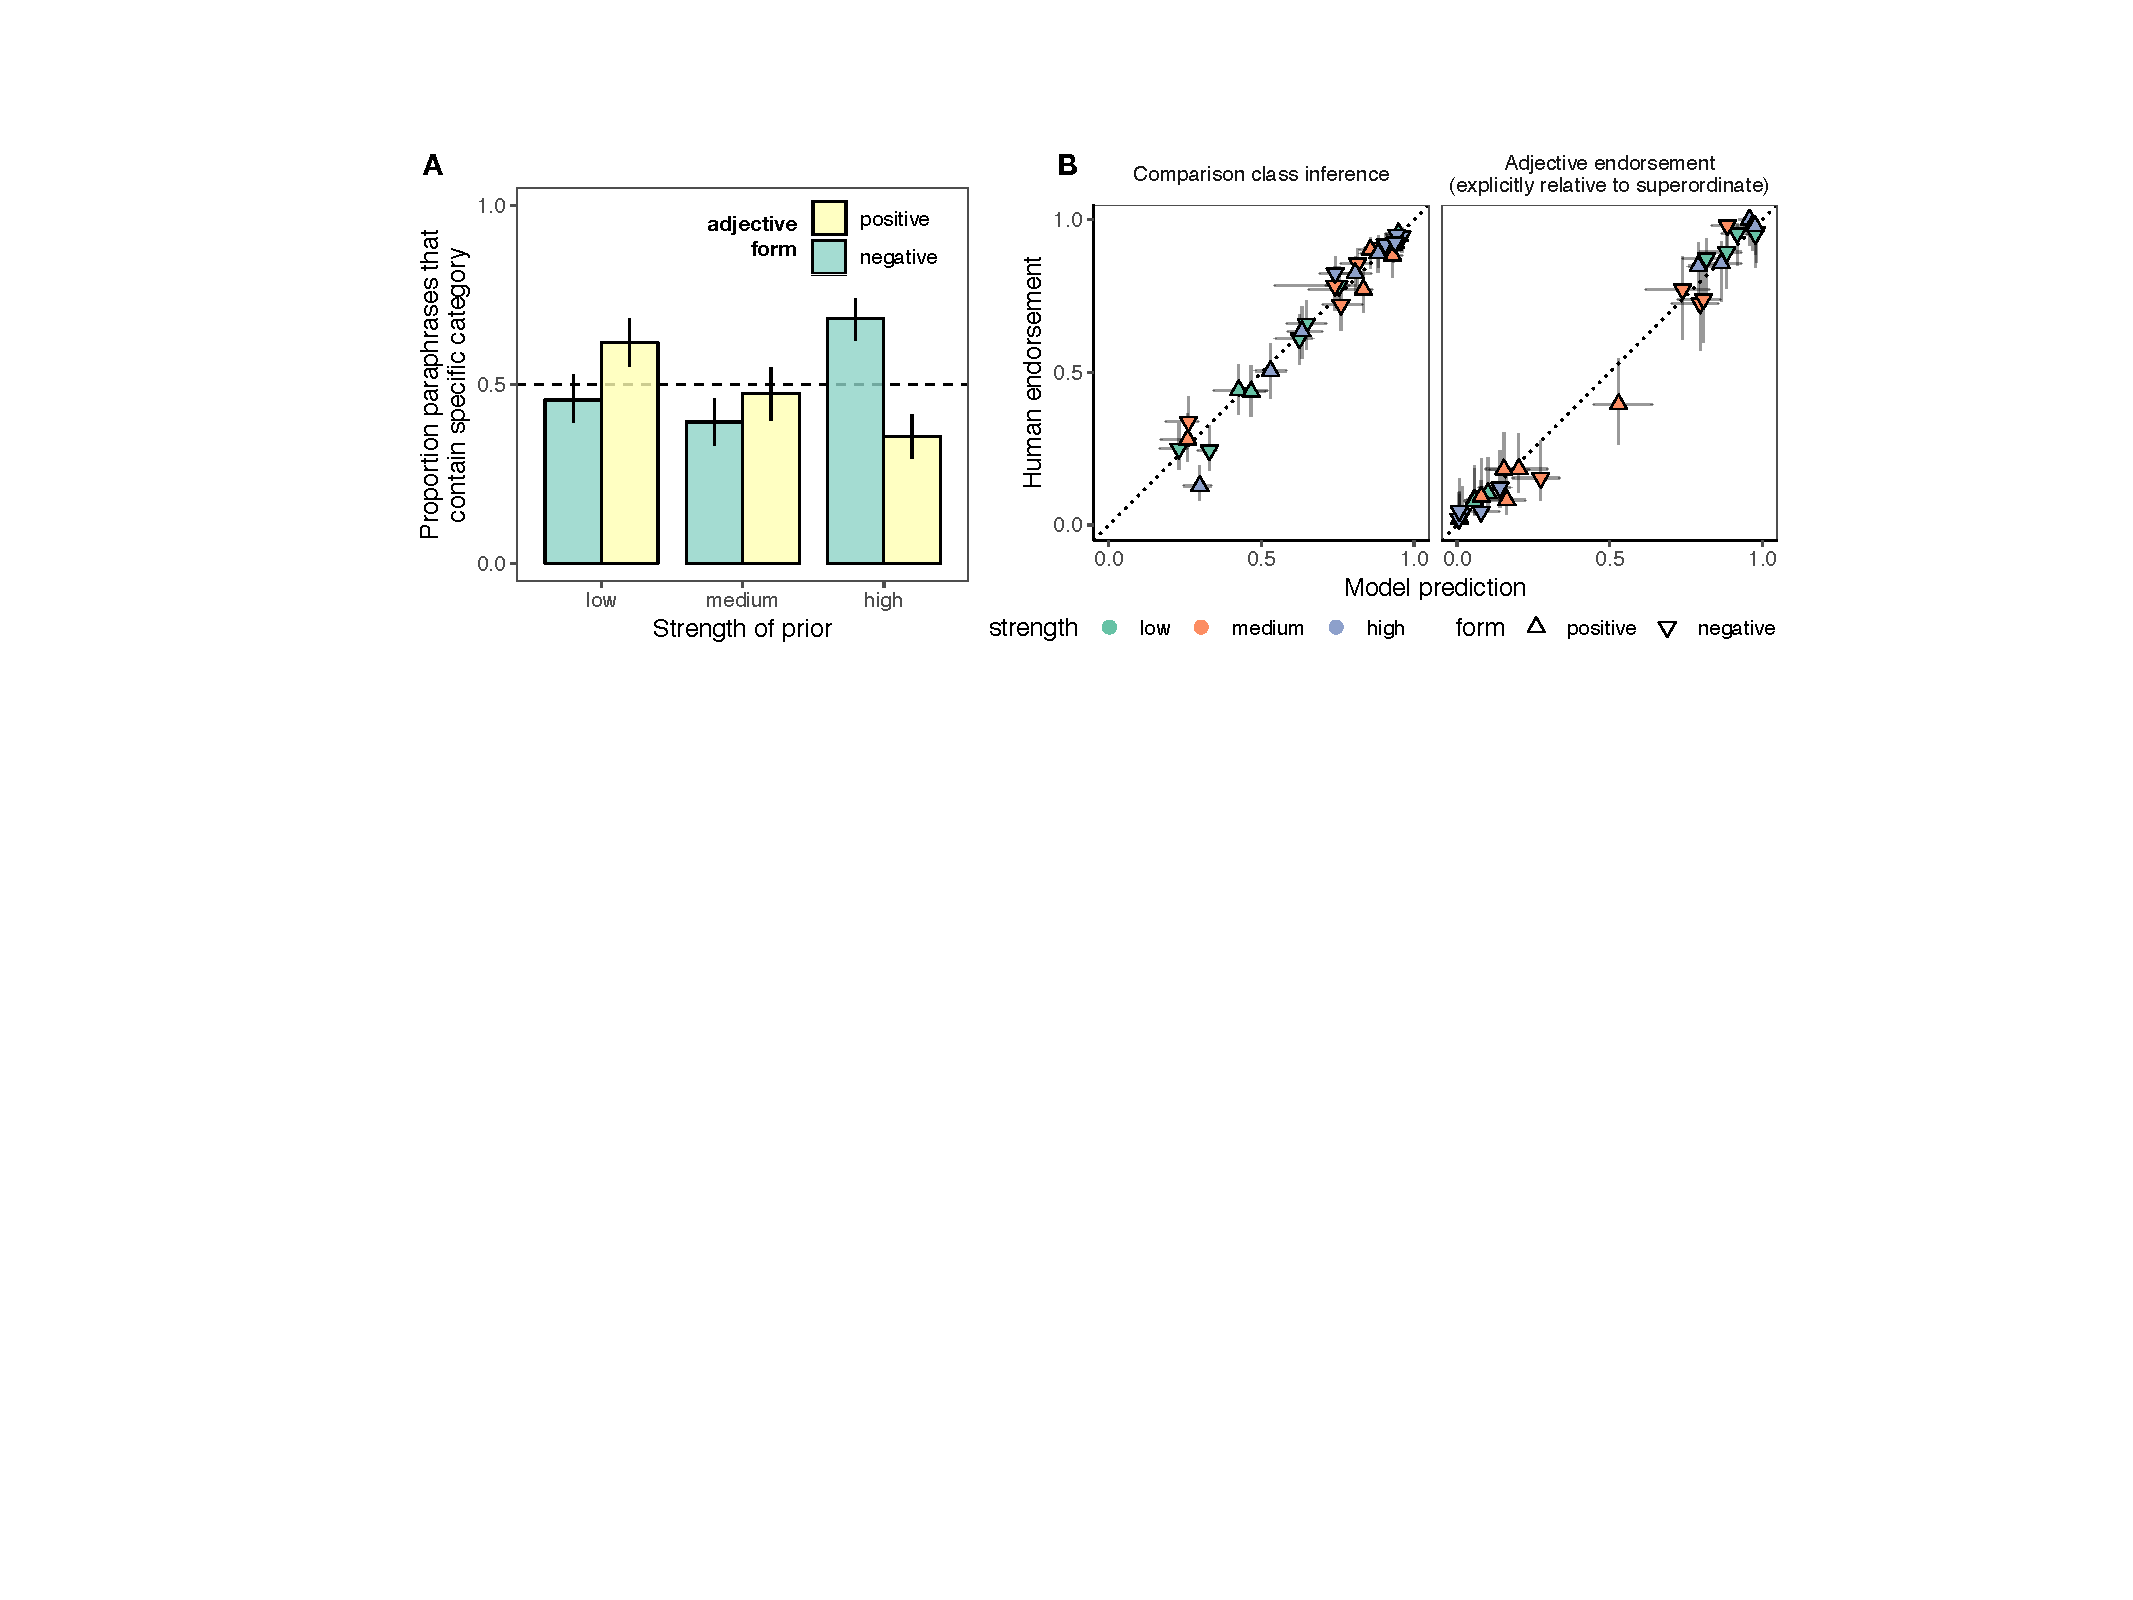
\includegraphics[width=0.9\textwidth]{bars_scatters}
  \end{center}
  \vspace{-0.55cm}
  \caption{\small  A: Human production of subordinate comparison classes averaged across items. X-axis orders different subordinate categories by their intuitive average value relative to a superordinate category 
  %for the relevant degree 
  (e.g., ``low'' = Winter; ``high'' = Summer; degree = temperature).
  B: Model fits for the two-alternative comparison class inference task (left) and adjective endorsement task (right). Error bars = 95\% credible intervals.}
  \label{fig:results}
    \vspace{-0.55cm}
\end{figure}


The free production data show the richness of the human capacity to reconstruct context.
An expensive crystal flower vase could be expensive for a \emph{crystal flower vase}, a \emph{flower vase}, a \emph{vase}, or just for an \emph{item} or \emph{gift}. 
As a simple test of our main hypothesis (Fig.~\ref{fig:predictions}), we coded each response as to whether or not the text contained the specific category (e.g., did the response mention the words \emph{crystal}, \emph{flower}, and \emph{vase}? did the response for a warm day in Winter mention \emph{winter}?), and we assume that responses which do not mention the specific  category refer to more general categories.
The qualitative predictions of the model (described above) were borne out (Fig.~\ref{fig:results}A).
% The relevant comparison class for items from specific categories that are expected to fall low the degree scale (``low'' strength of prior e.g., a day in Winter) is expected to be the specific category (\emph{winter}) when a positive adjective (\emph{warm}) but not a negative adjective is used (\emph{cold}); the reverse effect is observed for items that are expected to fall high on the degree scale (``high'' strength of prior).

To test the quantitative predictions of the model, we designed a two-alternative forced choice version of the experiment ($n=264$). The model's predictions depend on both the relative prior distributions over the degree scale (e.g., temperatures of days in Winter vs. over the year) and the prior distribution over comparison classes. 
As an extremely rough approximation for the prior over comparison classes, we take the corpus frequency of the noun phrase. 
To infer the priors over the degrees, we ran an additional adjective endorsement task ($n=100$) where participants are asked to judge if an adjective applied to a typical member of the subordinate category (e.g., a typical day in Winter) explicitly relative to the more general category (e.g., cold relative to a typical day of the year). 
We then used a Bayesian data analytic model together with an RSA model for adjective endorsement to triangulate the priors over the degrees that would accommodate both data sets.
The model provides a strong quantitative fit to the comparison class inference data (Fig.~\ref{fig:results}B), demonstrating that these inferences can be investigated with quantitative methods.

%When processing a conjunctive phrase, listeners may form expectations about the complete utterance even before the sentence is over. 
%For example, when a speaker reaches the word \emph{and} in ``Elephants live in Africa \emph{and}'', she has two syntactically distinct options available to her when completing the sentence: She could continue with a noun phrase (e.g., ``and Asia'') or a verb phrase (e.g., ``and eat bugs'').
%Each of these continuations would imply different inferences about the prevalence of elephants in Africa.\footnote{
%	Of course, it is possible to continue with a verb phrase about a mutually exclusive property such as ``\ldots live in Africa and live in Asia'' as well as continue with a noun phrase about a non-mutually exclusive property (e.g., ``\ldots eat figs and nuts''). Our focus is on the fact that a speaker can continue the conjunction with a mutually exclusive or non-mutually exclusive property, which in the cases we consider, are highly correlated with NP~vs.~VP coordination.
%}
%If listeners parse and interpret utterances incrementally at the level of individual words, then we would expect their 



%\begin{wrapfigure}{r}{0.5\textwidth}
%\vspace{-1cm}
%  \begin{center}
%    \includegraphics[width=0.48\textwidth]{expt2_summary}
%  \end{center}
%  \vspace{-1cm}
%  \caption{\small Experiment 1 results.  Participants rate prevalence for mentioned property (\% live in Africa) and ``Property 2'', either the mutually exclusive property (left two bars) or non-mutually exclusive property (right two bars). ``\_\_'' indicates the question appears mid-sentence. Error-bars denote bootstrapped 95\% confidence intervals.}
%  \label{fig:expt1}
%\end{wrapfigure}



%\begin{wrapfigure}{l}{0.5\textwidth}
%\vspace{-1cm}
%  \begin{center}
%    \includegraphics[width=0.48\textwidth]{expt3_summary}
%  \end{center}
%  \caption{\small Experiment 2 results. Participants are interrupted at various stages of the sentence (either after \emph{Africa}, \emph{and}, or \emph{Asia}) to be asked about the prevalence of \emph{living in Africa} and \emph{living in some other place}, or asked at the end of the sentence (right-most bars). When participants are interrupted before the second conjunct (\emph{Asia}), the sentence continues with a non-mutually exclusive property. Error-bars denote bootstrapped 95\% confidence intervals.
%}
%\vspace{-1cm}
%\label{fig:expt2}
%\end{wrapfigure}



%We tested the incremental prediction of the model that when participants only hear ``Elephants live in Africa and'', they will begin to anticipate a mutually-exclusive conjunct, and that this would manifest in their implied prevalence ratings being substantially less than when they only hear ``Elephants live in Africa''.





\vspace{-0.3cm}

\begingroup
\renewcommand{\section}[2]{}
\bibliographystyle{apacite}

\setlength{\bibleftmargin}{.125in}
\setlength{\bibindent}{-\bibleftmargin}

\bibliography{../paper/comparison-class}
\renewcommand\bibname{}
\scriptsize
%Extending an analysis of generics to handle complex-predicates poses unique challenges.
%A sentence of the form ``Ks F and G'' introduces an ambiguity:
%
%\begin{enumerate}
%\tightlist
%\item $\denote{gen}(K) [F \land G]$
%\item $\denote{gen}(K) [F] \land \denote{gen}(K) [G]$
%\end{enumerate}
\endgroup

\end{document}
